\documentclass[conference,a4paper,twoside]{IEEEtran}
\usepackage[utf8x]{inputenc}
\usepackage{ucs}
\usepackage{amsmath}
\usepackage{amsfonts}
\usepackage{amssymb}
\usepackage{graphicx}
\usepackage{url}
\usepackage{hyperref}
\author{Daniel Thomas}
\begin{document}
\title{Security of deployed Android devices}


% author names and affiliations
% use a multiple column layout for up to three different
% affiliations
\author{
\IEEEauthorblockN{Daniel R.\ Thomas,
Daniel Wagner,
Alastair R.\ Beresford,
Andrew Rice}
\IEEEauthorblockA{
Computer Laboratory\\
University of Cambridge\\
Cambridge, United Kingdom\\
Firstname.Lastname@cl.cam.ac.uk
}
}


\maketitle


\begin{abstract}
Android is the most popular smartphone platform and seeks to provide better security than popular desktop operating systems through increased compartmentalisation and a permission system for apps.
This security relies on there not being root privilege exploits which allow apps to bypass all protections.
Many such exploits have been found and fixed.
Our hypothesis is that these fixes do not promptly reach the users devices and so much of the time users are running versions of Android known to be vulnerable.
We used the DeviceAnalyzer data\cite{TODO} and found that on average over XX\% of devices were exposed to known vulnerabilities. %TODO (drt24) proportion of devices exposed on average.
There was also a period of several months when no devices ran secure versions of Android.
\end{abstract}

\section{Introduction}
Android has XX\% of the smartphone market~\cite{TODO} and while the core development is controlled by Google there are at least XX~\cite{TODO} manufacturers which make devices which run Android.
Many of these manufacturers customise the version of Android they ship and sometimes network operators (of which there are at least XX~\cite{TODO}) make further modifications.
Hence when Google produces an update to Android, the update may have to pass through the manufacturer and operator before reaching the user.
The manufacturer and user have no financial incentive to perform this work.
There is ongoing legal action to force some of them to do so~\cite{TODO}.

Android relies on the Linux kernel to provide compartmentalisation and runs each app as a separate unix `user'.
The Linux kernel is a large piece of software and so there will always be new root exploits found in it~\cite{TODO}.
Manufacturers of Android devices have also added further root exploits when customising it~\cite{TODO}.
Between XX\%~\cite{TODO} and XX\%~\cite{TODO} of malware for Android contains root exploits.
While this shows that much Android malware does not need a root exploit to work, it can just request the relevant permissions and the user will grant them, a significant proportion does.
This malware is also more dangerous because while ordinary malware can be remotely removed by Google through the Play store, once a root exploit has been used there are no guarantees.

Figure \ref{fig:proportioninsecure} shows the proportion of Android devices in the DeviceAnalyzer data which were running versions of Android known to root exploits at the time.
In \S\ref{sec:background} we will explain where these data comes from and then in \S\ref{sec:results} we will show these data in more detail.


\begin{figure}[!b]
\centering
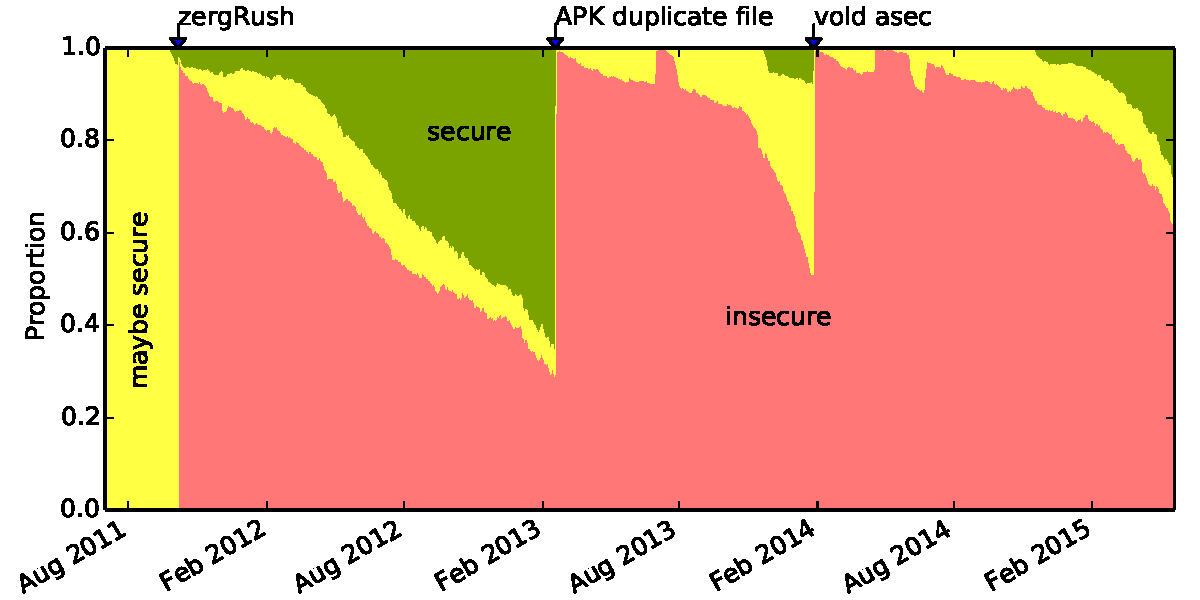
\includegraphics[width=\columnwidth]{figures/proportioninsecure}
%TODO make this graph shorter
\caption{Proportion of devices running insecure versions of android}
\label{fig:proportioninsecure}
\end{figure}

\section{Background}
\label{sec:background}
There are two sources of data we needed for this study, information on root exploits and information on installed versions of Android.

\subsection{Root exploits}
We compiled a list of root exploit vulnerabilities for Android containing information on when they were known about, what versions they affected and which versions fixed the problem.
We only looked for \emph{root equivalent} exploits which did not require USB debugging to exploit.
\emph{Root equivalent} means that it grants privileges equivalent in scope to root which can then be used to gain root.
Some phones can be `rooted' by enabling USB debugging and using the special privileges of the adb shell to root the device.
This is not something that applications running on the phone can exploit to break compartmentalisation and so we do not include those exploits.
Some exploits which grant root are not traditional kernel exploits, for example the discovery of flaws in the verification of signatures on Android applications in ??? 2013 meant that applications could pretend to be signed with system keys and hence gain root privileges.

We have published full details of the vulnerabilities listed below in an accompanying technical report~\cite{TODO} and summarise them in Table \ref{tab:andvulns}.
We also have a website\footnote{\url{TODO}} which we will keep up to date with future vulnerabilities.

\begin{table}
\centering
\begin{tabular}{c|c|c}
Vulnerability & Date known & How known \\
\hline
Exploid & 2010-07-15 & Public disclosure \\
Psneuter & 2011-01-06 & Public disclosure \\
Levitator & 2011-03-10 & CVE registered \\
ZergRush & 2011-10-06 & Exploit developed \\
APK duplicate file & 2013-02-18 & Fix committed \\
APK unsigned shorts & 2013-07-03 & Fix committed \\
% TODO this is an incomplete list, we need to add the rest here and in os-version.py
\end{tabular}
\caption{Root equivalent vulnerabilities in Android}
\label{tab:andvulns}
\end{table}

\subsection{Versions of Android running on devices}
We also need historical information on which versions of Android were running on devices along with other information about those devices which allows us to go into more detail and confirm the reliability of the data our results depend on.
The only suitable data which is available for this is the DeviceAnalyzer data~\cite{TODO}.
The DeviceAnalyzer data contains data from ??? devices with a total of ??? device days, it contains data for more than ??? months for ??? devices.
%TODO talk about the DeviceAnalyzer project a bit
Various different kinds of data\footnote{\url{TODO}} are collected by the DeviceAnalyzer Android app\footnote{\url{TODO}}.
Among these are the build string and API version for the version of Android currently running on the device each day.
The API/SDK version is a well defined integer, however it does not always change with new Android releases, particularly security bug fixes should not increase this value.
The build string is `The user-visible version string', fortunately most (99.9\%) devices in the data have a build string of the form `x.y.z random string' and so it is possible to extract the Android version number.

\subsection{Running a version of Android known to be vulnerable makes a device vulnerable}
While we have not tried to exploit these vulnerabilities on the devices in order to test whether the devices are actually vulnerable, we are confident that most devices.

\section{Results}
\label{sec:results}
In this section we present the results of our analysis showing ????. %TODO summarise our results

Figure \ref{fig:os} shows the raw data on the number of devices in the DeviceAnalyzer data running different versions of Android each day.
It shows how old versions are gradually replaced by new ones, the long tail of devices which do not see updates to more recent versions and the fluctuation in the number of devices in the data.
\begin{figure}%[!b]
\centering
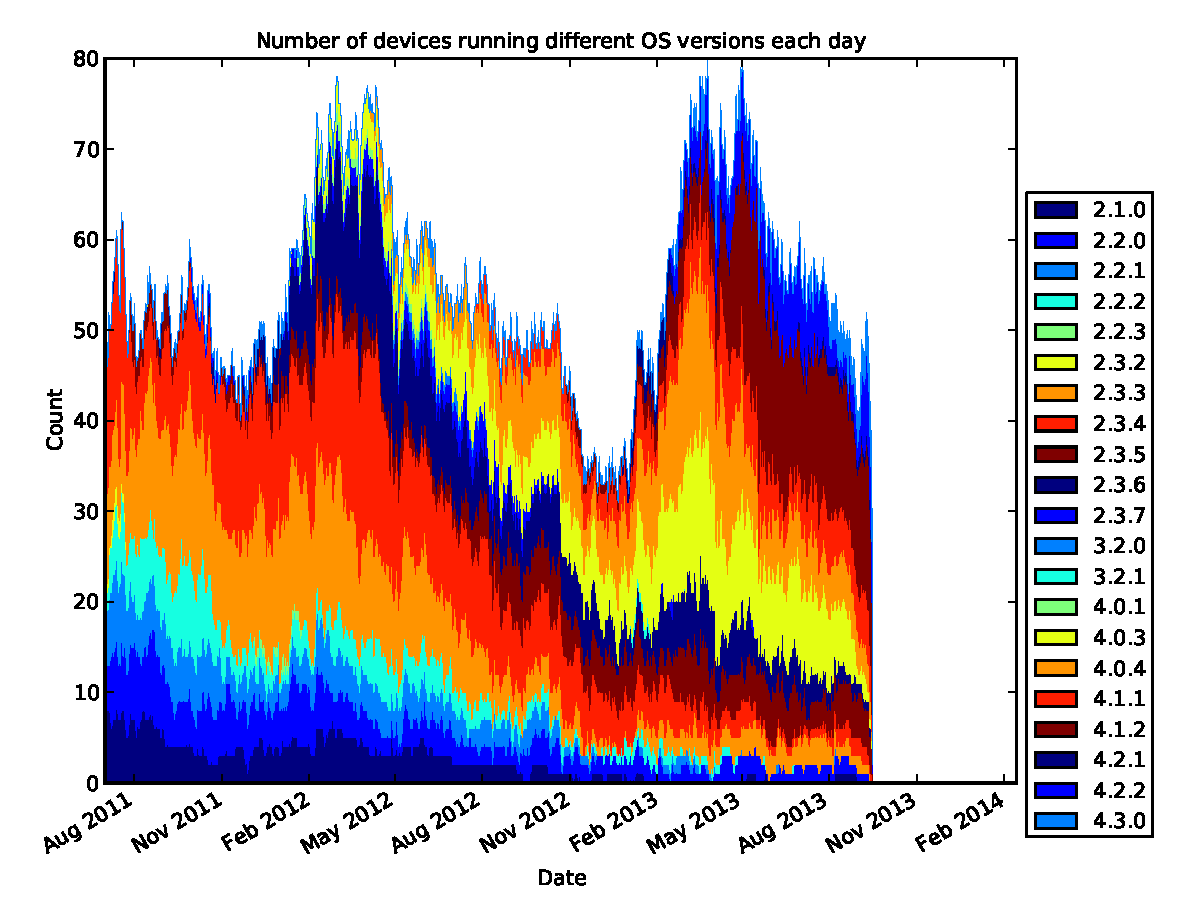
\includegraphics[width=\columnwidth]{figures/os}
\caption{Android versions in DeviceAnalyzer data over time}
\label{fig:os}
\end{figure}

Figure \ref{fig:vulnerabilities} shows which vulnerabilities devices are exposed to.
For each vulnerability it shows the proportion of devices exposed to that vulnerability and how that changes over time.
In July 2011 at the beginning of the DeviceAnalyzer data the Exploid and Levitator vulnerabilities both affect most Android devices, slowly these are fixed as updates roll out and devices are replaced until in January 2013 a much smaller proportion of devices are affected by known vulnerabilities.
However when in February 2013 the first APK signing vulnerability was found which affected all previous versions of Android and even in October 2013 most devices were still unfixed. %TODO put percentages on these things to quantify them
\begin{figure}%[!b]
\centering
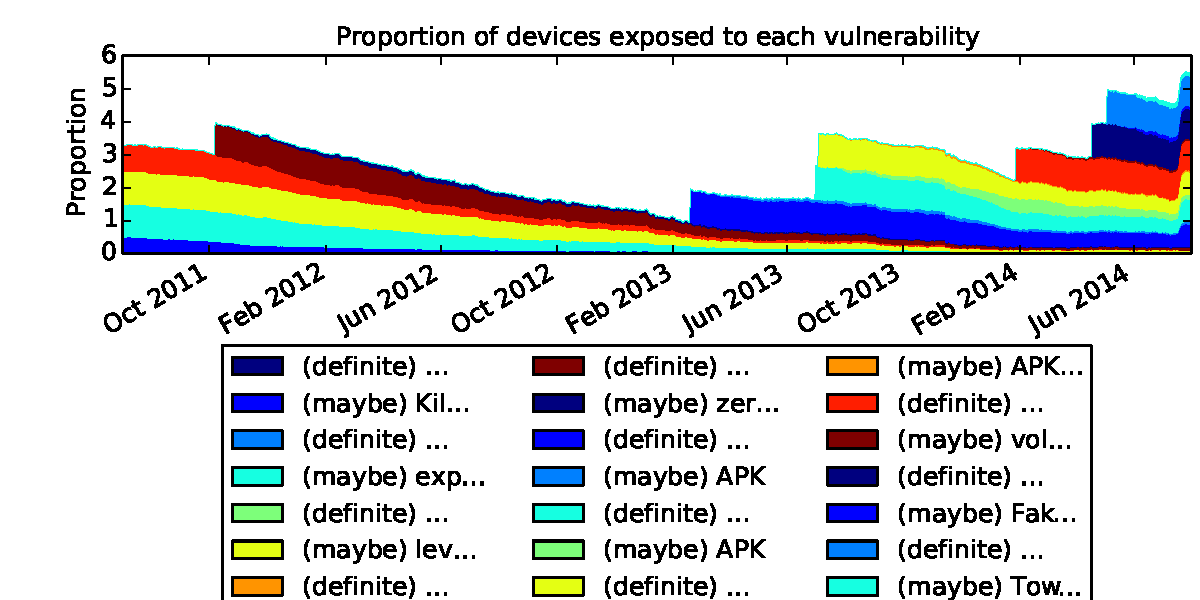
\includegraphics[width=\columnwidth]{figures/vulnerabilities}
\caption{Proportion of devices exposed to each vulnerability with time (1.0 is 100\%)}
\label{fig:vulnerabilities}
\end{figure}

\subsection{Update frequency}
%TODO find out what the frequency of updates is

\section{Related work}
\label{sec:related}
Stopping root exploits working: SEAndroid, Capsicum, iOS.
Detecting malware: Android antivirus useless.


\section{Conclusion}
\label{sec:conclusion}

\end{document}